\documentclass{ximera}

\pgfplotsset{my style/.append style={axis x line=middle, axis y line=
middle, xlabel={$x$}, ylabel={$y$}, axis equal }}


\title{Intro to Mathematical Reasoning}
\begin{document}
\begin{abstract}
Topic 1 Practice Problems
\end{abstract}
\maketitle

%%% Topic: Mathematical Reasoning. Subtopics:
%   Clarifying questions
%   Extraneous vs vital information/data
%   Information vs Data
%

\input{Useful-Validators}

%%%%%%%%%%%%%%%%%%%%%%%%%%%%%%%%%%%%%%%%%%%%%%%%%%%%%%%%%%%%%%%%%%%%%%%%%%%%%%%%%
%%%%%%%%%                        Question Code                           %%%%%%%%
%%%%%%%%%%%%%%%%%%%%%%%%%%%%%%%%%%%%%%%%%%%%%%%%%%%%%%%%%%%%%%%%%%%%%%%%%%%%%%%%%


\begin{problem}
    In a residential neighborhood most families have multiple cars; at least one for each parent and maybe one for the kids over 16. You have learned to recognize every car in your neighborhood and which house it belongs to. What is the domain of this association (recognizing the car and then recalling which house it belongs to)?
    \begin{multipleChoice}
        \choice{The houses in the neighborhood.}
        \choice{Your individual neighbors.}
        \choice[correct]{The cars in the neighborhood.}
    \end{multipleChoice}
    \begin{problem}
        What is the codomain?
        \begin{multipleChoice}
            \choice[correct]{The houses in the neighborhood.}
            \choice{Your individual neighbors.}
            \choice{The cars in the neighborhood.}
        \end{multipleChoice}
        \begin{problem}
            Is this association a function?
            \begin{multipleChoice}
                \choice{No, each house has multiple cars.}
                \choice{No, each car belongs to multiple people.}
                \choice[correct]{Yes, each car belongs to one house.}
                \choice{Yes, each house has one car.}
            \end{multipleChoice}
        \end{problem}
    \end{problem}
\end{problem}

\begin{problem}
    You decide to plant pines trees to provide a privacy screen around a piece of your property. Use the following information to answer the questions.
    \begin{itemize}
        \item You choose white pine as it is a fast-growing variety.
        \item At the time of planting, the trees are all 2 feet tall.
        \item The land you wish to screen is 14 feet by 20 feet.
        \item You think pine trees are quite pretty.
    \end{itemize}
    Which of these are pieces of data?
    \begin{selectAll}
        \choice {You choose white pine as it is a fast-growing variety.}
        \choice[correct] {At the time of planting, the trees are 2 feet tall.}
        \choice[correct] {The land you wish to screen is 14 feet by 20 feet.}
        \choice {You think pine trees are quite pretty.}
    \end{selectAll}

    \begin{problem}
        You would like to know how long it will take the trees to reach a sufficient height to screen your property from the road. Which pieces of information are relevant?
        \begin{selectAll}
            \choice [correct]{You choose white pine as it is a fast-growing variety; they grow an average of 2.7 feet per year.}
            \choice[correct] {At the time of planting, the trees are 2 feet tall.}
            \choice{The land you wish to screen is 14 feet by 20 feet.}
            \choice {You think pine trees are quite pretty.}
        \end{selectAll}

        \begin{problem}
            After looking up information you determine it is easiest to first figure out how high the trees will be each year, and then use that to determine how long you must wait. When writing a mathematical expression for this, what should the independent variable be?
            \begin{multipleChoice}
                \choice{The height of the trees.}
                \choice[correct]{The time in years.}
                \choice{The height of the trees at planting.}
            \end{multipleChoice}

            \begin{problem}
                Write an equation describing this relationship using $t$ for the time in years and $h$ for the height of the trees in feet. $\answer{h}$ = $\answer{2.7t+2}$

                \begin{problem}
                    Identify the domain, codomain, and whether this equation is a function.
                    \begin{multipleChoice}
                        \choice{\textbf{Domain: }height in feet; \\ \textbf{Codomain: }time in years; \\ \textbf{Is it a function? }yes}
                        \choice{\textbf{Domain: }time in years; \\ \textbf{Codomain: }height in feet; \\ \textbf{Is it a function? }no}
                        \choice{\textbf{Domain: }height in feet; \\ \textbf{Codomain: }time in years; \\ \textbf{Is it a function? }no}
                        \choice[correct]{\textbf{Domain: }time in years; \\ \textbf{Codomain: }height in feet; \\ \textbf{Is it a function? }yes}
                    \end{multipleChoice}
                \end{problem}
            \end{problem}
        \end{problem}
    \end{problem}
\end{problem}

\begin{problem}
    Does the following graph depict a function?
\begin{center}
    \begin{tikzpicture}
        \begin{axis}[my style, minor tick num=1]
            \addplot[domain=-3:5]{-abs(x-1)+3};
        \end{axis}
    \end{tikzpicture}
\end{center}

    \begin{multipleChoice}
        \choice[correct]{Function}
        \choice{Not a function}
    \end{multipleChoice}
\end{problem}


Use the following graph for Problems 4-7.
\begin{center}
    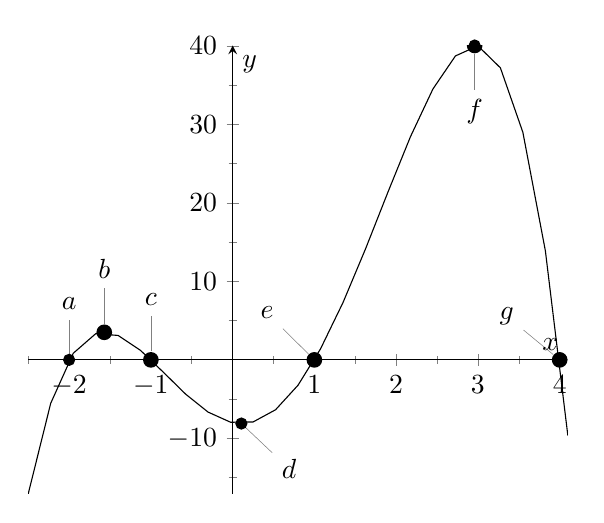
\begin{tikzpicture}[baseline={([yshift={-1ex}]current bounding box.north)}]
        \begin{axis}[axis x line=middle, axis y line=
        middle, xlabel={$x$}, ylabel={$y$}, minor tick num=1]
            \addplot[domain=-2.5:4.1]{-(x+1)*(x-1)*(x+2)*(x-4)};
            \addplot [mark=*, only marks] coordinates{(-1,0)(1,0)(-2,0)(4,0)(-1.57,3.51)(0.107,-8.11)(2.96,40.04)};
            \node[pin={90:{$a$}},circle,fill,inner sep=1pt] at (axis cs:-2,0) {};
            \node[pin={90:{$b$}},circle,fill,inner sep=2pt] at (axis cs:-1.57,3.51) {};
            \node[pin={90:{$c$}},circle,fill,inner sep=2pt] at (axis cs:-1,0) {};
            \node[pin={320:{$d$}},circle,fill,inner sep=1pt] at (axis cs:0.107,-8.11) {};
            \node[pin={135:{$e$}},circle,fill,inner sep=2pt] at (axis cs:1,0) {};
            \node[pin={270:{$f$}},circle,fill,inner sep=2pt] at (axis cs:2.96,40.04) {};
            \node[pin={145:{$g$}},circle,fill,inner sep=2pt] at (axis cs:4,0) {};
        \end{axis}
    \end{tikzpicture}
\end{center}

 \begin{problem}
     Is the function that is shown continuous?
     \begin{multipleChoice}
         \choice[correct]{Continuous}
         \choice{Not continuous}
     \end{multipleChoice}
\end{problem}

\begin{problem}
    Which points mark local extrema? (Select all that apply).
    \begin{selectAll}
        \choice{a}
        \choice[correct]{b}
        \choice{c}
        \choice[correct]{d}
        \choice{e}
        \choice[correct]{f}
        \choice{g}
    \end{selectAll}
    \begin{problem}
        Identify whether these points are maxima or minima.

        Point b is a
        \begin{multipleChoice}
            \choice[correct]{Maximum}
            \choice{Minimum}
        \end{multipleChoice}

        Point d is a
        \begin{multipleChoice}
            \choice{Maximum}
            \choice[correct]{Minimum}
        \end{multipleChoice}

        Point f is a
        \begin{multipleChoice}
            \choice[correct]{Maximum}
            \choice{Minimum}
        \end{multipleChoice}
    \end{problem}
\end{problem}

\begin{problem}
    Which points are absolute extrema? Select all that apply.
        \begin{selectAll}
            \choice{a}
            \choice{b}
            \choice{c}
            \choice{d}
            \choice{e}
            \choice[correct]{f}
            \choice{g}
        \end{selectAll}
    \begin{problem}
        Is this point a maximum or minimum?
        \begin{multipleChoice}
            \choice[correct]{Maximum}
            \choice{Minimum}
        \end{multipleChoice}
    \end{problem}
\end{problem}

\begin{problem}
    Identify the zeros of the function. (Select all that apply.)
    \begin{selectAll}
        \choice[correct]{a}
        \choice{b}
        \choice[correct]{c}
        \choice{d}
        \choice[correct]{e}
        \choice{f}
        \choice[correct]{g}
    \end{selectAll}
\end{problem}

\begin{problem}
    Does the following graph depict a function?

    \begin{tikzpicture}
        \begin{axis}[my style, minor tick num=1]
            \addplot[domain=-3:3](x*x,x);
        \end{axis}
    \end{tikzpicture}

    \begin{multipleChoice}
        \choice{Function}
        \choice[correct]{Not a function}
    \end{multipleChoice}
\end{problem}

\begin{problem}
    Use the plot to answer the questions.

    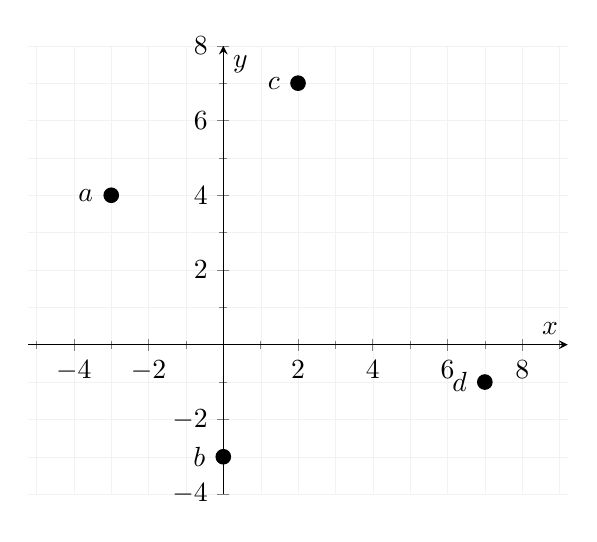
\begin{tikzpicture}
        \begin{axis}[my style,grid=both,
    grid style={line width=.1pt, draw=gray!10}, minor tick num=1, ymax=8, ymin=-4]

            \addplot[mark=*,only marks] coordinates {(-3,4)(0,-3)(2,7)(7,-1)};
            \node[label={180:{$a$}},circle,fill,inner sep=2pt] at (axis cs:-3,4) {};
            \node[label={180:{$b$}},circle,fill,inner sep=2pt] at (axis cs:0,-3) {};
            \node[label={180:{$c$}},circle,fill,inner sep=2pt] at (axis cs:2,7) {};
            \node[label={180:{$d$}},circle,fill,inner sep=2pt] at (axis cs:7,-1) {};
        \end{axis}
    \end{tikzpicture}

    What are the coordinates of point $a$? ($\answer{-3}$,$\answer{4}$)

    What are the coordinates of point $b$? ($\answer{0}$,$\answer{-3}$)

    What are the coordinates of point $c$? ($\answer{2}$,$\answer{7}$)

    What are the coordinates of point $d$? ($\answer{7}$,$\answer{-1}$)
\end{problem}

Match the graph manipulations to the appropriate \textbf{parent functions} (\textbf{NOTE: }not the actual function of the graph, but the parent function of the graph).

A) 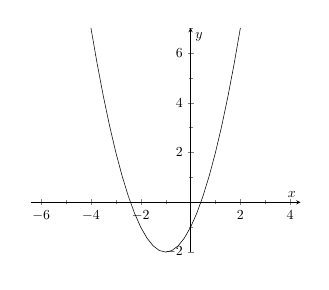
\begin{tikzpicture}[baseline={([yshift={-1ex}]current bounding box.north)}, scale=0.50]
    \begin{axis}[my style, minor tick num=1]
        \addplot[domain=-4:2]{3(x+1)^2-2};
    \end{axis}
\end{tikzpicture}
B) \begin{tikzpicture}[baseline={([yshift={-1ex}]current bounding box.north)}, scale=0.50]
    \begin{axis}[my style, minor tick num=1]
        \addplot[domain=-12:3]{2^(x+1) - 1};
    \end{axis}
\end{tikzpicture}

C) \begin{tikzpicture}[baseline={([yshift={-1ex}]current bounding box.north)}, scale=0.50]
    \begin{axis}[my style, minor tick num=1, xmin=0]
        \addplot[domain=1:5]{sqrt(x-1)};
    \end{axis}
\end{tikzpicture}
D) \begin{tikzpicture}[baseline={([yshift={-1ex}]current bounding box.north)}, scale=0.50]
    \begin{axis}[my style, minor tick num=1]
        \addplot[domain=-5:3]{4/5*x +2};
    \end{axis}
\end{tikzpicture}

E) \begin{tikzpicture}[baseline={([yshift={-1ex}]current bounding box.north)}, scale=0.50]
    \begin{axis}[my style, minor tick num=1]
        \addplot[domain=-3:3]{ln(x)};
    \end{axis}
\end{tikzpicture}
F) 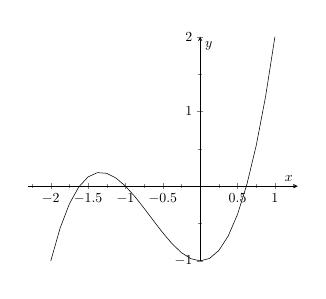
\begin{tikzpicture}[baseline={([yshift={-1ex}]current bounding box.north)}, scale=0.50]
    \begin{axis}[my style, minor tick num=1]
        \addplot[domain=-2:1]{x^3+2*x^2-1};
    \end{axis}
\end{tikzpicture}

\begin{problem}
    Which graph would most properly be said to have a parent function of $f(x) = x^2$

    Plot: $\answer{A}$
\end{problem}
\begin{problem}
    Which graph would most properly be said to have a parent function of $f(x) = \sqrt{x}$

     Plot: $\answer{C}$
\end{problem}
\begin{problem}
    Which graph would most properly be said to have a parent function of $f(x) = x$

    Plot: $\answer{D}$
\end{problem}
\begin{problem}
   Which graph would most properly be said to have a parent function of $f(x) = e^x$

    Plot: $\answer{B}$
\end{problem}
\begin{problem}
    Which graph would most properly be said to have a parent function of $f(x) = x^3$

    Plot: $\answer{F}$
\end{problem}
\begin{problem}
    Which graph would most properly be said to have a parent function of $f(x) = \ln(x)$

    Plot: $\answer{E}$
\end{problem}


\end{document}